\documentclass[handout]{beamer}
\usepackage[T1]{fontenc}
\usepackage[utf8]{inputenc}
\usepackage{lmodern}
\usepackage[italian]{babel}

\title{Account Google}
\author{Mattia Cozzi}
\date{a.f.~2024/2025}


%\documentclass[handout]{beamer}     %usare questa classe per generare l'handout

%\usepackage{pdfpages}   %per mostrare più quadri nella stessa pagina
%\pgfpagesuselayout{4 on 1}[a4paper,border shrink=5mm,landscape]


\usetheme{Singapore}
%\useoutertheme[left]{sidebar} %elementi intorno alle diapositive
\setbeamercovered{dynamic} %modifica l'aspetto del testo grigetto delle diapositive future. Argomenti: invisible/transparent/dynamic


%COLORE PRINCIPALE
\definecolor{verde}{RGB}{2, 194, 117} % UBC Blue (primary)
\setbeamercolor{structure}{fg=verde} % itemize, enumerate, etc
\setbeamercolor{alerted text}{fg=verde}


\usecolortheme{orchid}

\usepackage{tikz}

\begin{document}

\begin{frame}
  \titlepage
\end{frame}


\begin{frame}
\frametitle{Contenuti}
\tableofcontents
\end{frame}



\section{Panoramica}


\begin{frame}
\frametitle{}

\end{frame}




\section{Gmail}

\begin{frame}
\frametitle{}

\end{frame}



\section{Contatti}

\begin{frame}
\frametitle{}

\end{frame}


\section{Calendar}

\begin{frame}
\frametitle{Cos'è Google Calendar}
Google Calendar è l'\alert{agenda elettronica} della suite Google.\pause

~

\begin{columns}
\begin{column}{.7\textwidth}
  Permette di:
  \begin{itemize}
    \item gestire i propri appuntamenti;\pause
    \item gestire gli appuntamenti di un gruppo di persone;\pause
    \item programmare eventi ricorrenti;\pause
    \item programmare videochiamate;\pause
    \item creare eventi a cui invitare partecipanti esterni.
  \end{itemize}  
\end{column}
\begin{column}{.2\textwidth}
  \begin{figure}
    
\includegraphics[width=\columnwidth]{img/calendarlogo.png}
  \end{figure}
\end{column}
\end{columns}
\end{frame}


\begin{frame}
\frametitle{Interfaccia principale}
\begin{figure}
  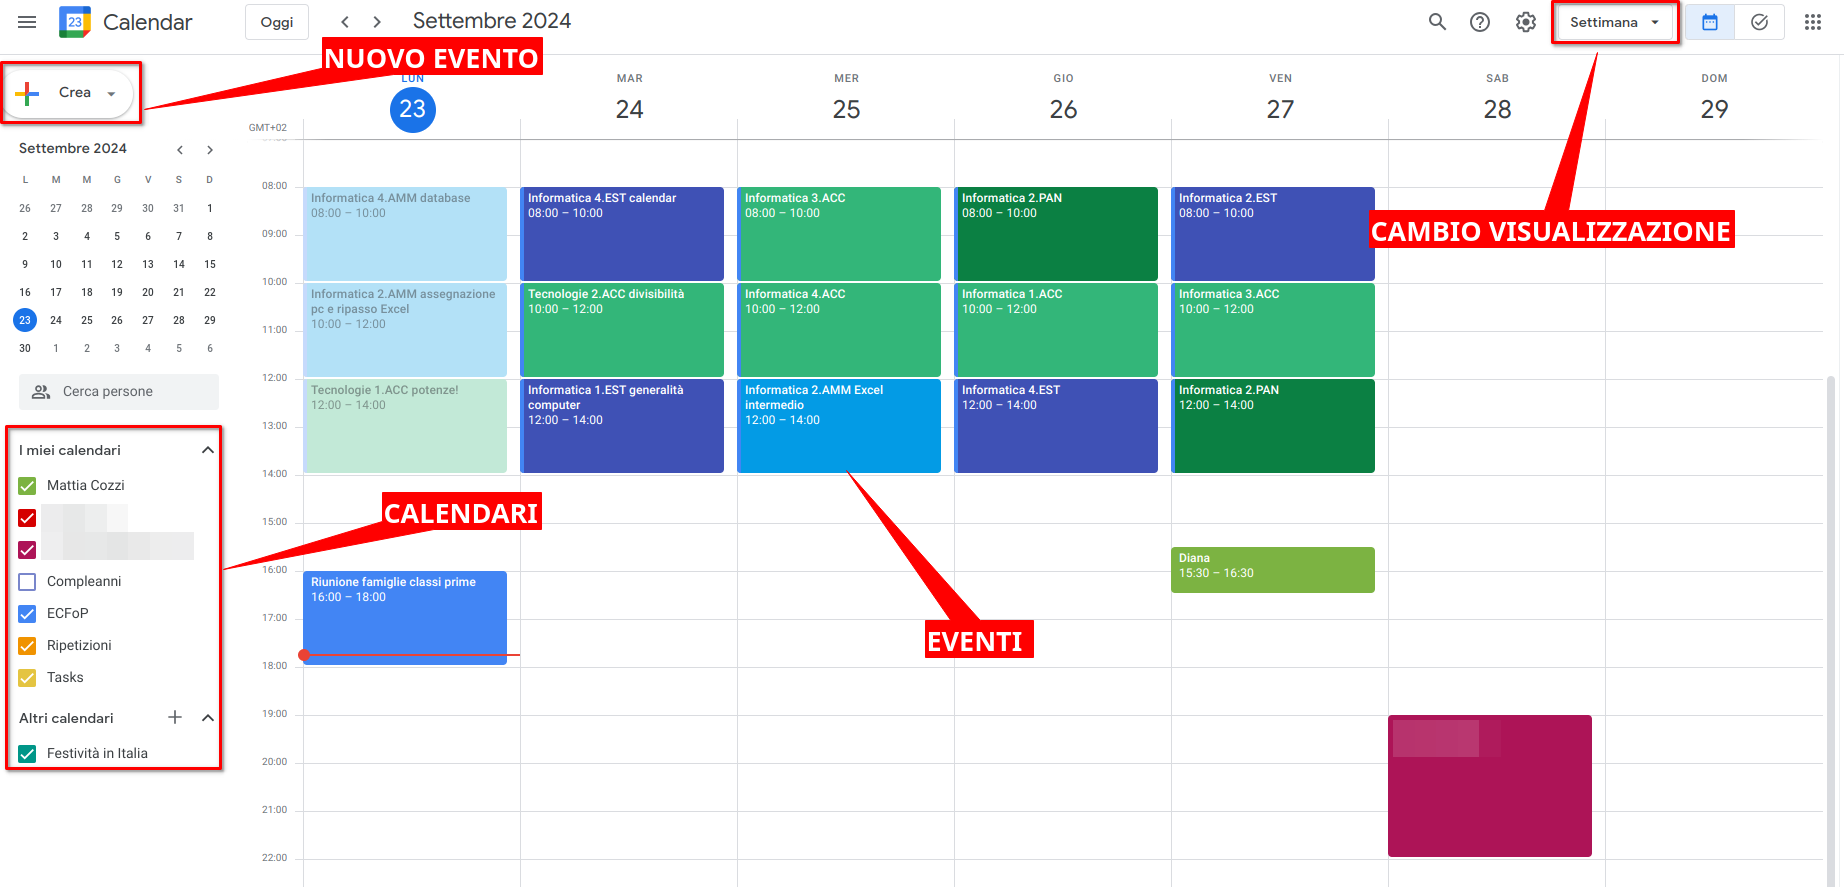
\includegraphics[width=\columnwidth]{img/calendar1.png}
\end{figure}
\end{frame}

\begin{frame}
\frametitle{Opzioni di visualizzazione}
\begin{figure}
  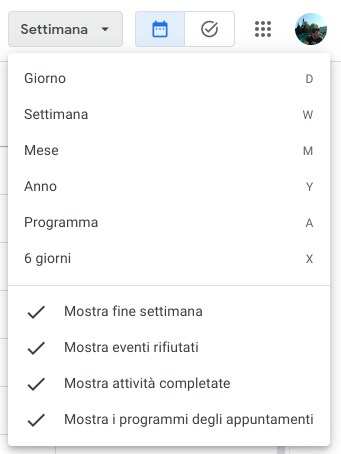
\includegraphics[width=.35\columnwidth]{img/calendarvisua.png}
\end{figure}

~

È possibile cambiare la porzione di tempo visualizzata.\pause

~

Attenzione alle scorciatoie!
\end{frame}


\begin{frame}
\frametitle{Creazione di un evento}
\begin{figure}
  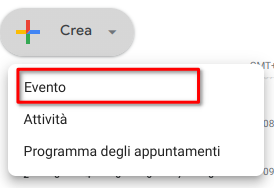
\includegraphics[width=.3\columnwidth]{img/calendarcrea.png}
\end{figure}
Apriamo la \alert{finestra rapida} di creazione evento.
\end{frame}



\begin{frame}
\frametitle{Finestra rapida creazione evento}
Questa finestra contiene alcune opzioni per la creazione di un nuovo evento, ma non tutte.

\begin{figure}
  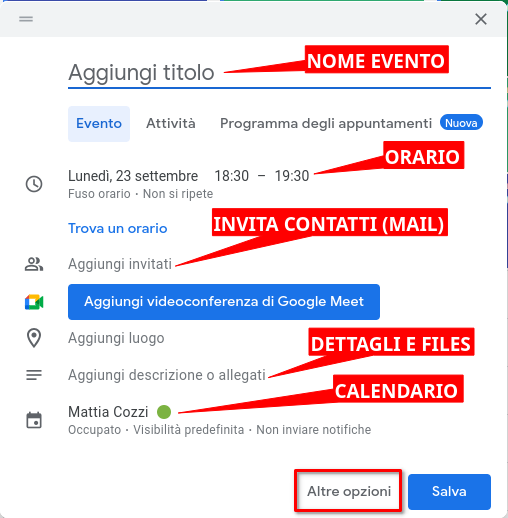
\includegraphics[width=.5\columnwidth]{img/calendarcrea2.png}
\end{figure}
\end{frame}

\begin{frame}
\frametitle{Invitati}
Scrivendo degli indirizzi email nello spazio per gli invitati, si condivide l'evento che stiamo creando con qualcuno.

~

Gli invitati ricevono una mail di invito, da cui possono decidere se accettare o meno. Se accettano, vedranno l'evento nel proprio calendario.

~

Quando si invita qualcuno, Calendar aggiunge automaticamente l'opzione per una videochiamata tramite Google Meet.
\end{frame}


\begin{frame}
\frametitle{Descrizione}
Molto utile la descrizione dell'evento, che può essere usata per:
\begin{columns}
  \begin{column}{.5\textwidth}
\begin{itemize}
  \item appunti;
  \item ordini del giorno di una riunione;
  \item file utili (posso allegare ricette mediche ad un appuntamento col dottore);
  \item commenti degli utenti coinvolti nell'evento.
\end{itemize}
  \end{column}
  \begin{column}{.4\textwidth}
    \begin{figure}
      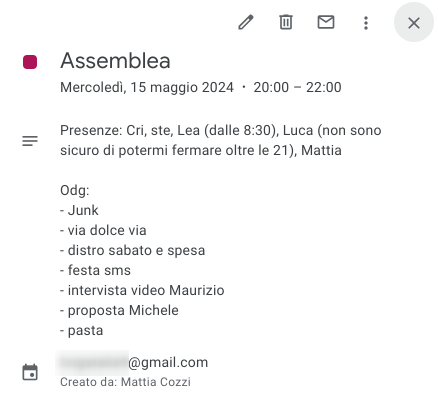
\includegraphics[width=\columnwidth]{img/calendarnotes.png}
    \end{figure}
  \end{column}
\end{columns}

\end{frame}


\begin{frame}
\frametitle{Modifica di un evento}
Una volta creato un evento, possiamo cambiarne il colore o eliminarlo facendo destro clic sull'evento.

\begin{figure}
  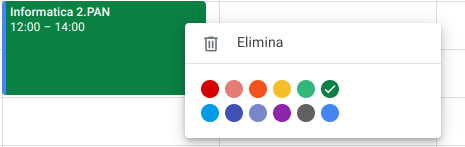
\includegraphics[width=.6\columnwidth]{img/calendarcolore.png}
\end{figure}

Trascinando i bordi di un evento possiamo inoltre modificarne graficamente la durata.

~

Trascinando l'evento posso spostarlo nel tempo.
\end{frame}



\begin{frame}
\frametitle{Più calendari}
Google Calendar può gestire diversi calendari contemporaneamente.

~

\begin{columns}
  \begin{column}{.5\textwidth}
    Organizzare il proprio lavoro con diversi calendari è utile per:
\begin{itemize}
  \item separare diverse attività: lavoro, studio, tempo libero;\pause
  \item gestire il calendario di più dipendenti/collaboratori;\pause
  \item condividere eventi con amici e parenti.
\end{itemize}
  \end{column}
  \begin{column}{.4\textwidth}
    \begin{figure}
      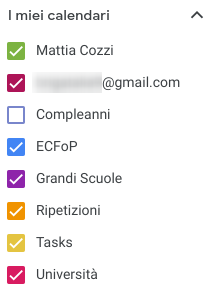
\includegraphics[width=\columnwidth]{img/calendarcals.png}
    \end{figure}
  \end{column}
\end{columns}
\end{frame}


\begin{frame}
\frametitle{Creazione di un calendario}
\begin{figure}
  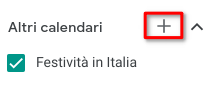
\includegraphics[width=.2\columnwidth]{img/calendarnuovocal.png}
\end{figure}
Per creare un nuovo calendario, clicchiamo sul + vicino ad ``Altri calendari''.

\begin{figure}
  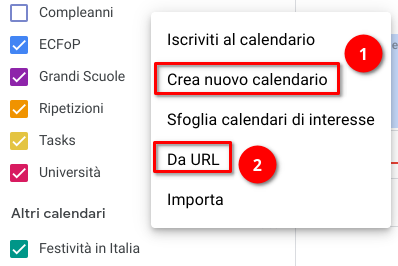
\includegraphics[width=.4\columnwidth]{img/calendarnuovocal2.png}
\end{figure}
L'opzione ``Da URL'' permette di iscriversi ad un calendario a cui siamo stati invitati tramite link (URL è sinonimo di link).
\end{frame}


\begin{frame}
\frametitle{Opzioni calendario}
Una volta creato un calendario, possiamo modificarne le proprietà cliccando sui tre puntini a fianco al nuovo calendario nell'interfaccia principale.

\begin{figure}
  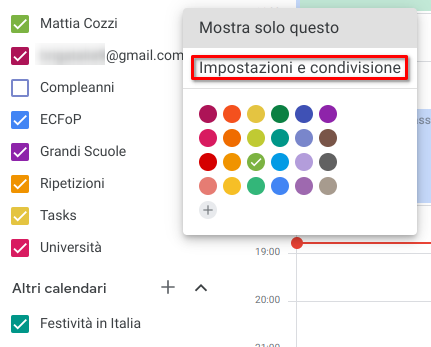
\includegraphics[width=.5\columnwidth]{img/calendarcalmod.png}
\end{figure}
\end{frame}



\begin{frame}
\frametitle{Condivisione di un calendario}
Dalla finestra delle opzioni calendario:
\begin{figure}
  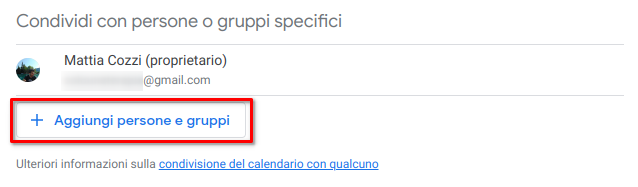
\includegraphics[width=.5\columnwidth]{img/calendarshare.png}
\end{figure}

\begin{columns}
  \begin{column}{.5\textwidth}
    \begin{figure}
      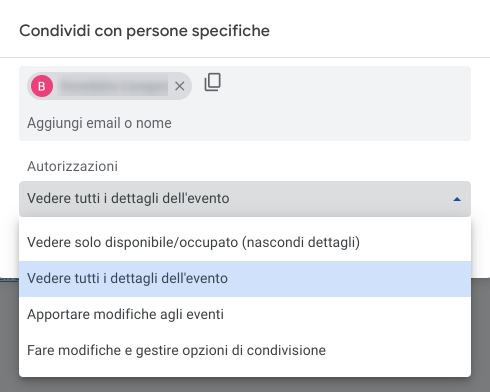
\includegraphics[width=\columnwidth]{img/calendarshare2.png}
    \end{figure}
  \end{column}
  \begin{column}{.4\textwidth}
    Un invitato può avere permessi (cioè ``poteri'') diversi.

    ~

    Gli invitati ricevono una mail, da cui possono decidere se accettare l'invito. Se sì, vedranno il nuovo calendario insieme ai loro.
  \end{column}
\end{columns}
\end{frame}

\begin{frame}
\frametitle{Finestra completa creazione evento}
La apriamo cliccando su ``Altre opzioni'' nella finestra rapida di creazione evento.

\begin{figure}
  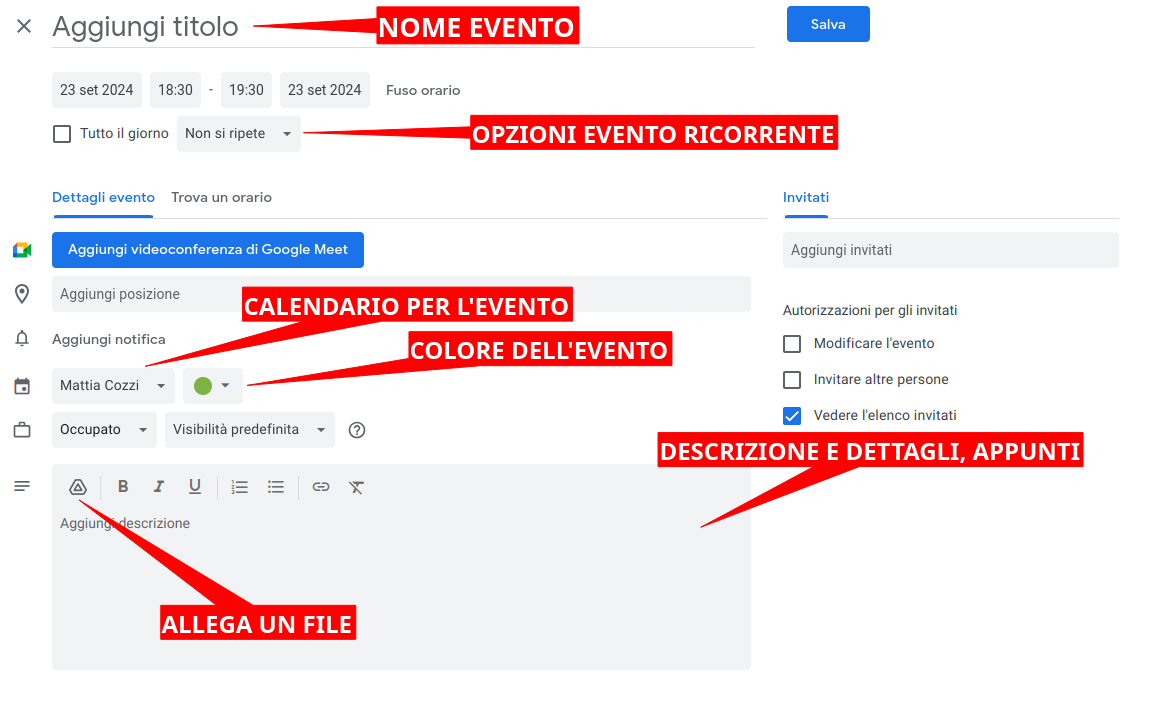
\includegraphics[width=\columnwidth]{img/calendarevento.png}
\end{figure}
\end{frame}

\begin{frame}
\frametitle{Eventi ricorrenti}
Spesso un evento si ripete nel tempo, come ad esempio:
\begin{itemize}
  \item un orario scolastico \begin{center}``tutti i lunedì alle 11 c'è matematica''\end{center}\pause
  \item un cliente ricorrente \begin{center}``la signora Rossi viene tutti i venerdì alle 10.30''\end{center}\pause
  \item un'attività ripetitiva \begin{center}``bagnare le piante ogni 10 giorni''\end{center}\pause
  \item un corso di qualche tipo \begin{center}``il corso di ceramica è  formato da 10 incontri tutti i lunedì sera, a partire dal 23 settembre''\end{center}\pause
\end{itemize}

~

Calendar contiene utilissime funzioni per gestire gli eventi ricorrenti.
\end{frame}

\begin{frame}
\frametitle{Impostazione eventi ricorrenti}
Possiamo impostare la ripetizione di un evento dalla pagina (anche rapida) di modifica evento:
\begin{figure}
  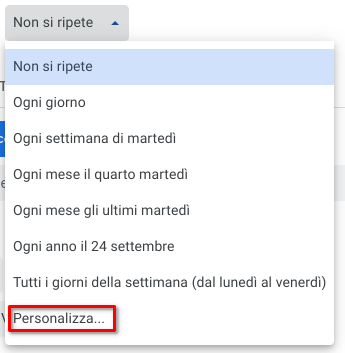
\includegraphics[width=.4\columnwidth]{img/calendarricorrente.png}
\end{figure}
Le opzioni più interessanti si trovano su ``Personalizza''.
\end{frame}


\begin{frame}
\frametitle{Esercizi}
\begin{enumerate}
  \item Crea un'agenda per la gestione di uno studio estetico o di acconciatura con le seguenti caratteristiche:
  \begin{itemize}
    \item tre calendari diversi (con anche colori diversi) per tre diversi collaboratori/collaboratrici dello studio;
    \item se riesci, invita dei tuoi compagni a partecipare come collaboratori (avrai bisogno dei loro indirizzi email);
    \item una settimana di appuntamenti piena, per tutti e tre collaboratori, dalle 9.00 alle 17.00;
    \item appuntamenti della durata da un'ora a due ore;
    \item pausa pranzo dalle 13.00 alle 14.00 (lasciare senza eventi).
  \end{itemize}
\end{enumerate}
\end{frame}

\begin{frame}
  \frametitle{Esercizi}
  \begin{enumerate}\setcounter{enumi}{1}
    \item Completa l'agenda precedente aggiungendo:
    \begin{itemize}
      \item una breve descrizione per ogni evento;
      \item un allegato (PDF o immagine) per ogni evento del martedì;
      \item ripetizione per 10 volte per almeno 5 appuntamenti.
      \item ripetizione fino a fine giugno per almeno 3 appuntamenti.
    \end{itemize}
  \end{enumerate}
\end{frame}

\begin{frame}
  \frametitle{Esercizi}
  \begin{enumerate}\setcounter{enumi}{2}
    \item Aggiungi all'agenda creata in precedenza gli eventi che puoi dedurre dalle seguenti email ricevute (sostituisci XXX e YYY con quello che ritieni più opportuno).
    
    ~

    \begin{itemize}
      \item Buongiorno, vorrei prenotare un trattamento XXX con la vostra estetista/parrucchiera YYY per venerdì prossimo. Io posso arrivare per le 11.00, in un'ora circa dovrei aver finito.

      Grazie e buona giornata, Anna

      ~
      \item Ciao a tutte, confermo la mia disponibilità a collaborare con il vostro studio tutti i martedì e i venerdì mattina, dalle 9.00 fino alla pausa pranzo. Potete iniziare a considerarmi nella vostra programmazione. Posso iniziare già la prossima settimana, e sarò disponibile a collaborare con voi fino alla metà di luglio.

      Attenzione: sarò assente dal lavoro il primo martedì di maggio e l'ultimo venerdì di giugno, per via di impegni personali.

      Ciao e a presto, Valentina
    \end{itemize}
  \end{enumerate}
\end{frame}






\section{Drive}

\begin{frame}
\frametitle{}

\end{frame}




\section{Maps}

\begin{frame}
\frametitle{}

\end{frame}


\section{Forms}

\begin{frame}
\frametitle{}

\end{frame}



\end{document}
